\documentclass[a4paper, 12pt]{article} % тип документа

%%%Библиотеки
	%\usepackage[warn]{mathtext}	
	\usepackage[T2A]{fontenc}   %Кодировка
	\usepackage[utf8]{inputenc} %Кодировка исходного текста
	\usepackage[english, russian]{babel} %Локализация и переносы
	\usepackage{caption}
	\usepackage{listings}
	\usepackage{amsmath, amsfonts, amssymb, amsthm, mathtools}
	\usepackage[warn]{mathtext}
	\usepackage[mathscr]{eucal}
	\usepackage{wasysym}
	\usepackage{graphicx} %Вставка картинок правильная
	\DeclareGraphicsExtensions{.pdf,.png,.jpg}
	\graphicspath{ {images/} }
	
	\setlength{\parskip}{0.5cm}
	
	\usepackage{pgfplots}
	\usepackage{indentfirst}
	\usepackage{float}    %Плавающие картинки
	\usepackage{wrapfig}  %Обтекание фигур (таблиц, картинок и прочего)
	\usepackage{fancyhdr} %Загрузим пакет
	\usepackage{lscape}
	\usepackage{xcolor}
	\usepackage[normalem]{ulem}
	\usepackage{wasysym}
	
	\usepackage{titlesec}
	\titlelabel{\thetitle.\quad}

	\usepackage{hyperref}
	\newenvironment{comment}{}{}

%%%Конец библиотек

%%%Настройка ссылок
	\hypersetup
	{
		colorlinks = true,
		linkcolor  = blue,
		filecolor  = magenta,
		urlcolor   = blue
	}
%%%Конец настройки ссылок


%%%Настройка колонтитулы
	\pagestyle{fancy}
	\fancyhead{}
	\fancyhead[L]{2.4.1}
	\fancyhead[R]{Старченко Иван, группа Б01-005}
	\fancyfoot[C]{\thepage}
%%%конец настройки колонтитулы

\begin{document}

%\maketitle
%\thispagestyle{empty}

%\newpage
\setcounter{page}{1}



\begin{center}
  \LARGE{Лабораторная работа 3.3.4}\\[0.2cm]
  \LARGE{Эффект Холла в полупроводниках.}\\[0.2cm]
  \large{10 сентября 2021 г.}\\[0.2cm]
  \large{Старченко Иван Александрович}\\[0.2cm]
\end{center}

\textbf{Цель работы:} \\
Измерение подвижности и концентрации носителей заряда в полупроводниках.

\textbf{В работе используются:} \\
Электромагнит с источником питания, батарейка, амперметр, реостат, цифровой вольтметр, милливеберметр, образцы легированного германия.
 


	\section{Экспериментальная установка.}
	Схема экспериментальной установки показана на рис. 2.
	
	\begin{figure}[h!]
		\centering
		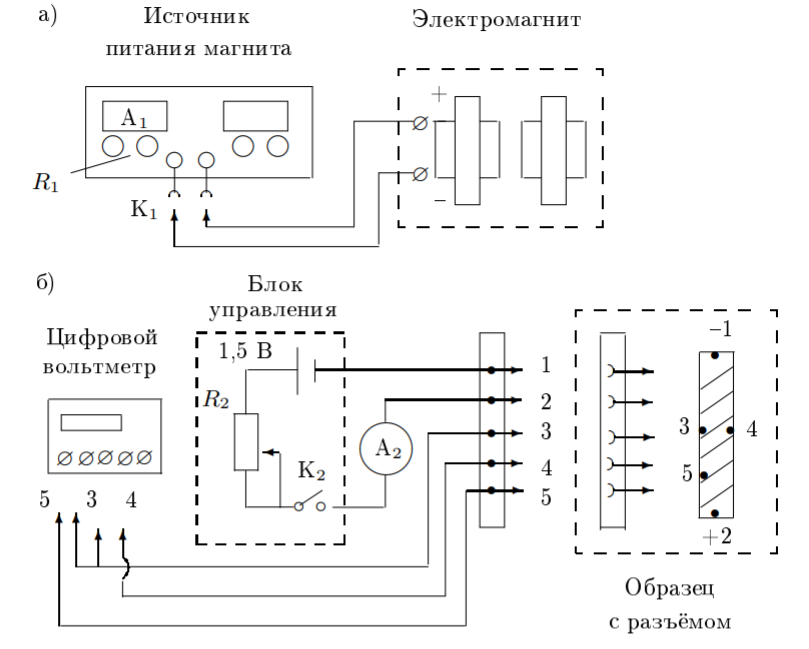
\includegraphics[width=\linewidth]{1}
		\caption{Схема установки для исследования эффекта Холла в полупроводниках}
		\label{fig:Holl2}
	\end{figure}
  
  	В зазоре электромагнита (рис. 1а) создаётся постоянное магнитное поле, величину которого можно менять с помощью регуляторов источника питания. Ток измеряется амперметром источника питания $A_{1}$. Разъем $K_{1}$ позволяет менять направление тока в обмотках электромагнита.
  
  	Образец из легированного германия, смонтированный в специальном держателе (рис. 1б), подключается к батарее. При замыкании ключа $K_{2}$ вдоль длинной стороны образца течет ток, величина которого регулируется реостатом $R$ и измеряется миллиамперметром $А_{2}$.
  	
  	В образце с током, помещённом в зазор электромагнита, между контактами 3 и 4 возникает разность потенциалов $U_{34}$, которая измеряется с помощью цифрового вольтметра.
  	
  	Контакты 3 и 4 вследствие неточности подпайки не всегда лежат на одной
  	эквипотенциали, и тогда напряжение между ними связано не только с эффектом
  	Холла, но и с омическим падением напряжения, вызванным протеканием основного тока через образец.
  	
  	Измеряемая разность потенциалов при одном направлении
  	магнитного поля равна сумме ЭДС Холла и омического падения напряжения, а
  	при другом  их разности. В этом случае ЭДС Холла $\mathscr{E}_{X}$ может быть определена как половина алгебраической разности показаний вольтметра, полученных для
  	двух противоположных направлений магнитного поля в зазоре.
  	
  	Можно исключить влияние омического падения напряжения иначе, если при каждом токе через образец измерять напряжение между точками 3 и 4 в отсутствие магнитного поля. При фиксированном токе через образец это дополнительное к ЭДС Холла напряжение $U_{0}$ остается неизменным. От него следует (с учетом
  	знака) отсчитывать величину ЭДС Холла: 
  	
  	$$\mathscr{E}_{X} = U_{34} \pm U_{0}$$. 
  	
  	При таком способе измерения нет необходимости проводить повторные измерения с противоположным направлением магнитного поля.
  	
  	
  	По знаку $\mathscr{E}_{X}$ можно определить характер проводимости - электронный или дырочный. Для этого необходимо знать направление тока в образце и направление
  	магнитного поля.
  	
  	Измерив ток $I$ в образце и напряжение $U_{35}$ между контактами 3 и 5 в отсутствие магнитного поля, можно, зная параметры образца, рассчитать проводимость материала образца по формуле:
  	
  \begin{equation}\label{sigma}
  	\sigma=\dfrac{I\cdot L_{35}}{U_{35}\cdot a\cdot l}
  \end{equation}
  	
  	где $L_{35}$ - расстояние между контактами 3 и 5, $a$ - толщина образца, $l$ - его ширина.


\section{{Ход работы}}

1) Проведём калибровку электромагнита. Для этого снимем зависимость магнитной индукции $B$, пронизывающего катушку в поле, от тока $I_M$. Результаты занесём в таблицу, а также представим на графике. 
    
2) Проведём измерение ЭДС Холла. Снимем зависимость напряжения $U_{3-4}$ от тока через обмотки магнита (с учётом $U_0$ при $I_M = 0$). Выполним серию экспериментов для различных токов через образец $I$ (от $0.3$ до $0.8$ мА). Результаты измерений занесём в таблицу, построим на одном графике семейство прямых.

3) Рассчитаем коэффициенты наклона семества графиков из предыдущщего пункта и занесем в таблицу.
    

\begin{table}[h]
    \centering
\begin{tabular}{|c|c|c|c|c|c|c|c|}\hline
$I_M, mA$ & 0.3 & 0.4 & 0.5 & 0.6 & 0.7 & 0.8\\ \hline
$k, \dfrac{\text{мВ}}{\text{Вб}}$ & 0.59 & 1.37 & 2.05 & 2.77 & 3.47 & 4.17\\ \hline
\end{tabular}\\
 \caption{\text{Коэффициент наклона при разных $I_M$}}
\end{table}

4) Построим график $k(I)$ и найдем коэффиуиент наклона графика, затем посчитаем $R_H$
\[R_{H} = \dfrac{h}{I}\cdot \dfrac{U}{B} = (106.8 \pm 0.2) \cdot 10^{-6} \dfrac{\text{м}^3}{\text{Кл}}\]

5) Посчитаем концентрацию $n$:
\[n = \frac{1}{R_H \cdot e} = (585 \pm 2)\cdot 10^{20} \frac{1}{\text{м}^3}\]

6) Посчитаем удельную проводимость материала $\sigma$:
\[\sigma = \frac{I\cdot L_{3-5}}{U_{3-5}\cdot h\cdot l} = (490 \pm 1)\cdot \frac{1}{Om m}\]

7) Вычислис подвижность $\mu$:
\[\mu = \sigma \cdot R_H = (519 \pm 9) \frac{\text{см}^2}{B\cdot c}\]

\section{{Вывод}}


Мы изучили явление эффекта Холла в полупроводниках, измерили для нашего образца (Германий) такие величины как постоянная Холла, концентрацию электронов, удельную проводимость и подвижность электронов.



\section{{Список используемой литературы}}

$\bullet$ \href{https://vk.com/doc-139677307_612194888}{Никулин М.Г. Лабораторный практикум по общей физике. Электричество и магнетизм}\\

$\bullet$ \href{https://mipt.ru/education/chair/physics/S_III/lab_el.php}{Описание лабораторных работ на кафедре общей физики МФТИ}

$\bullet$ \href{https://vk.com/doc-139677307_612194961}{П.В. Попов, А.А. Нозик. Обработка результатов учебного эксперимента}

\newpage
 
\section{Графики}

\begin{figure}[h]
    \centering
    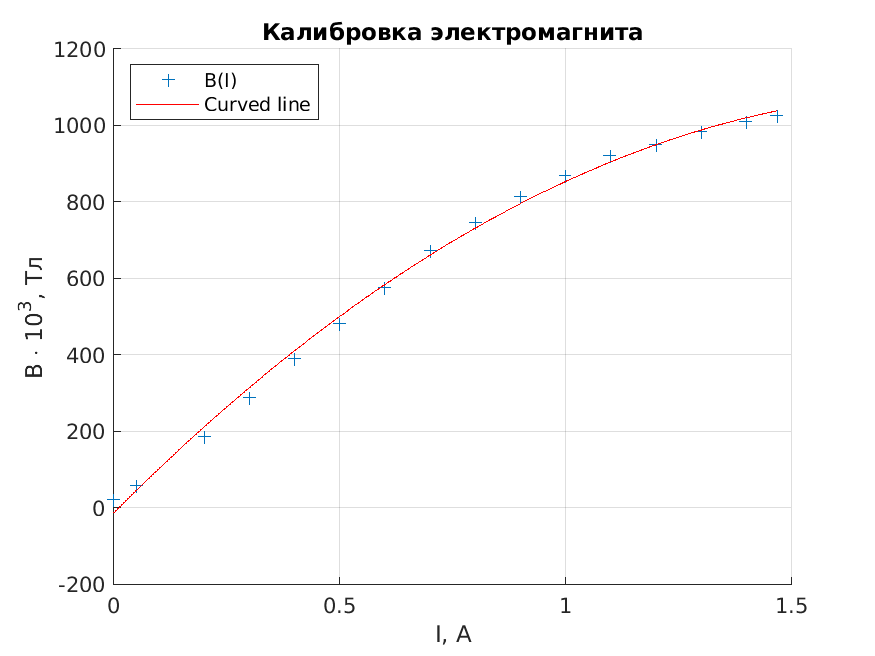
\includegraphics[width=1\textwidth]{graph1.png}    
    \caption{Калибровка электромагнита}
\end{figure}


\begin{figure}
    \centering
    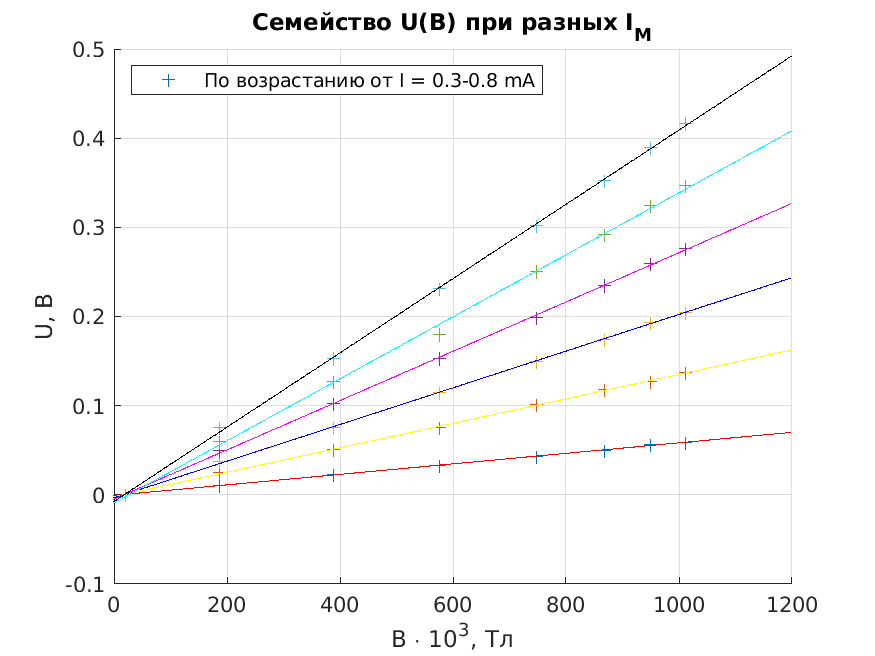
\includegraphics[width=1\textwidth]{graph2.png}    
    \caption{Семейство $U(B)$ при разных $I_M$}
\end{figure}


\begin{figure}
    \centering
    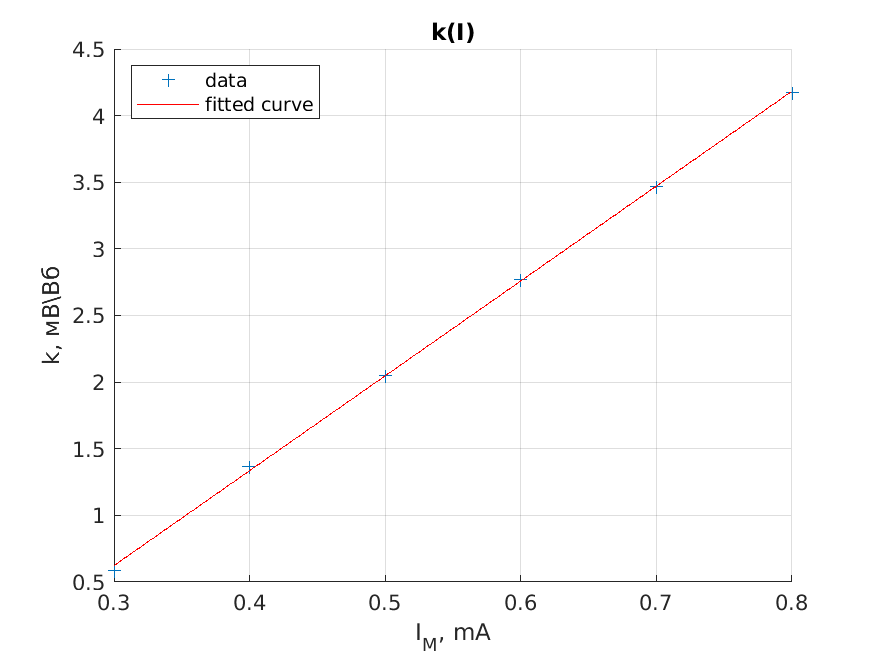
\includegraphics[width=1\textwidth]{graph3.png}    
    \caption{$k(I)$}
\end{figure}


\newpage

\section{Таблицы}

\begin{table}[h]
    \centering
    \begin{tabular}{|c|c|c|c|c|c|c|c|c|c|c|} \hline
$I_M, A$ & 0 & 0.1 & 0.2 & 0.3 & 0.4 & 0.5 & 0.6 & 0.7  \\ \hline
$B\cdot 10^{3}, $Вб & 20.8 & 57.5 & 186.9 & 289.6 & 389.3 & 481.7 & 576.7 & 671.5  \\ \hline

\end{tabular}\\

\begin{tabular}{|c|c|c|c|c|c|c|c|c|}\hline
$I_M, A$              & 0.8 & 0.9 & 1.0 & 1.1 & 1.2 & 1.3 & 1.4 & 1.47 \\ \hline
$B\cdot 10^{3}, $Вб  & 747.1 & 814.3 & 868.3 & 919.9 & 949.2 & 984.1 & 1011 & 1025.2\\ \hline
\end{tabular}\\
 \caption{Калибровка электромагнита}
\end{table}

\begin{table}[h]
    \centering
\begin{tabular}{|c|c|c|c|c|c|c|c|c|}\hline
$I_M, A$ & $B\cdot 10^3, \text{Вб}б$ & $I = 0.3,A$ & $I = 0.4,A$ & $I = 0.5 A$ & $I = 0.6,A$ & $I = 0.7,A$ & $I = 0.8,A$ \\ \hline
0 & 20.8 & 0 & 0 & 0 & 0 & 0 & 0 \\ \hline
0.2 & 186.9 & 0.011 & 0.025 & 0.037 & 0.05 & 0.06 & 0.075 \\ \hline
0.4 & 389.3 & 0.023 & 0.051 & 0.076 & 0.102 & 0.127 & 0.153 \\ \hline
0.6 & 576.7 & 0.033 & 0.076 & 0.115 & 0.153 & 0.18 & 0.231 \\ \hline
0.8 & 747.1 & 0.043 & 0.101 & 0.15 & 0.199 & 0.25 & 0.302 \\ \hline
1 & 868.3 & 0.05 & 0.118 & 0.174 & 0.235 & 0.292 & 0.353 \\ \hline
1.2 & 949.2 & 0.056 & 0.127 & 0.193 & 0.259 & 0.324 & 0.389 \\ \hline
1.4 & 1011 & 0.059 & 0.137 & 0.205 & 0.276 & 0.347 & 0.416 \\ \hline
\end{tabular}\\
 \caption{\text{Семейство $U(B)$ при разных $I_M$}}
\end{table}








 




\end{document}